\section{Scanner} \label{sec:Scanner}
Im Rahmen des Versuches sollen die Studierenden ihre Systeme auf Schwachstellen untersuchen. Diese ausfindig gemachten Schwachstellen sollen im Anschluss beseitigt werden. Eine Überwachung wird benötigt, um zu prüfen, ob die Studierenden diese Schwachstellen behoben haben. Das Abschalten, beziehungsweise die Verhinderung der Verwendung eines Dienstes, stellt in den meisten Fällen keine Behebung der Schwachstelle dar und wird deshalb ebenfalls geprüft. Um diese Überprüfung zu ermöglichen, wird ein Scanner benötigt, der die Dienste auf alle teilnehmenden \textit{GameClients} abfragt und auswertet. Die bei der Überprüfung gesammelten Daten werden benötigt, um die Servicepunkte der Gruppen zu berechnen.

\subsection{Verteilte Scanner}
Eine Idee für die Lastverteilung des Scanners ist ein verteilter Scanner. Hierbei wird ein Worker-Scanner auf jedem GameClient implementiert, welcher das eigene System überwacht. Ein Main-Scanner sammelt die von den Worker Scannern erstellten Ergebnisse ein und speichert diese in einer Datenbank ab. 

Der Vorteil des verteilten Scanners ist die Skalierbarkeit, da der Scanner auf dem Server nur von weiteren Scannern die Ergebnisse abholen, jedoch keine Überwachung durchführen muss.

Der verteilte Scanner bringt jedoch auch einige Nachteile mit sich. So muss sichergestellt werden, dass der Scanner auf dem User Client nicht manipuliert worden ist und die Ergebnisse valide sind. Eine solche Überprüfung könnte mithilfe eines \textquote{Fingerabdrucks} geschehen. Jedoch muss dann auch geprüft werden, ob das Programm zur Erstellung des Fingerabdrucks manipuliert worden ist.   Des Weiteren muss gewährleistet werden, dass der auf dem Client laufende Scanner dieselben Antworten und Ergebnisse erhält, wie ein fremder Nutzer. Dies ist notwendig, da die überwachten Services weiterhin von anderen Mitspielenden verwendet werden sollen.

Auf Grundlage der Nachteile, des Aufwandes der Implementierung und der ausreichenden Leistung des zentralen Scanners für den aktuellen Anwendungsfall wird ein verteilter Scanner nicht in Betracht gezogen. Die Idee des zentralen Scanners wird weiterverfolgt.

\subsection{Zentraler Scanner}
Die Herangehensweise des zentralen Scanners vermeidet die vorher beschriebenen Nachteile, da dem Ergebnis des Scanners vertraut werden kann und der Scanner zwangsläufig eine externe Sicht auf das System einnimmt. Das Ergebnis wird auf einem System ohne Einfluss der Mitspielenden berechnet.

\begin{center}
	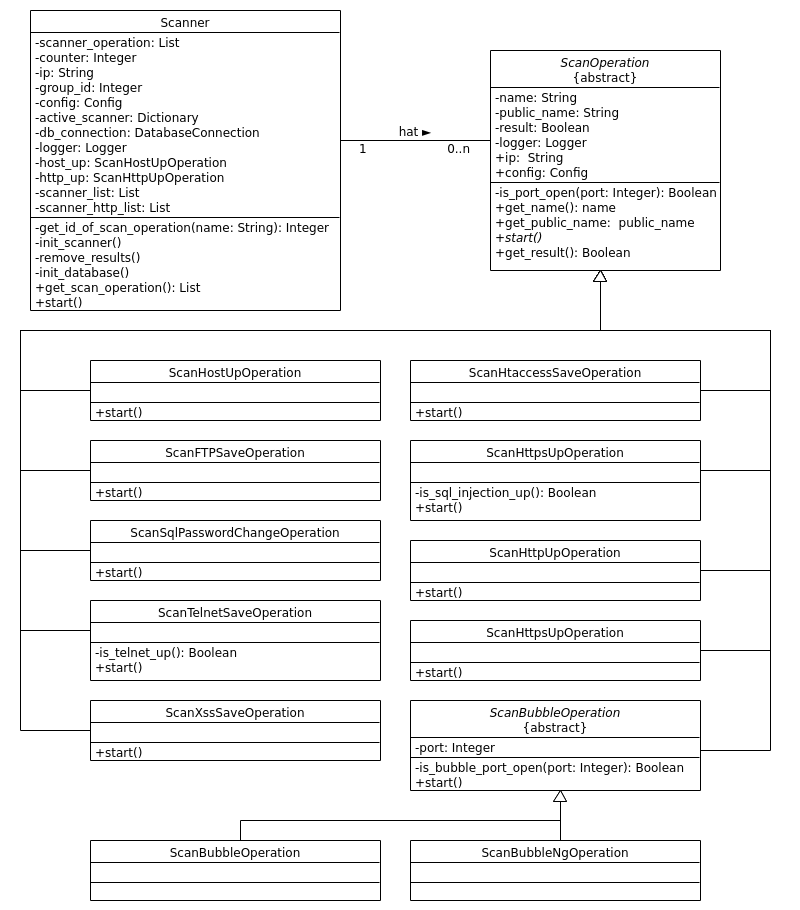
\includegraphics[width=\linewidth]{entwurf/scanner/class_scanner}
	\captionof{figure}{Klassen der Big Brother Komponente (Klassendiagramm)}
	\label{fig:scanner-class}
\end{center}

Wie in Bild \ref{fig:scanner-class} erkennbar besteht die Komponente Big Brother aus der Klasse Scanner, der abstrakten Klasse ScanOperation sowie den abgeleiteten Scan-Operationen.

Die Klasse \textit{ScanOperation} definiert die abstrakte Methode \textit{start()}. Diese wird von den abgeleiteten Klassen implementiert und ermöglicht das Starten der einzelnen Scan-Operationen. Ebenfalls speichern alle Scan-Operationen ihr Ergebnis im privaten Attribute \textit{result} ab. Mithilfe der von der abstrakten Klasse implementierten Methode \textit{get\_results()} kann der Scanner das Ergebnis der Scan-Operation auslesen. Jedes Objekt der Klasse Scanner startet 0 bis n Scan-Operationen abhängig von der Konfiguration beziehungsweise den aktiven Diensten. Des Weiteren stellt die abstrakte Klasse die Methode \textit{is\_port\_open()} bereit, welche von den Scan-Operationen genutzt werden kann, um den Status eines Ports auf dem fremden System zu prüfen. Ein Objekt der Klasse Scanner kann pro Typ maximal eine Scan-Operation starten und beinhaltet bzw. verwaltet alle Scan-Operationen für ein GameClient. 

Pro GameClient wird ein Objekt der Klasse Scanner für die Überwachung benötigt.

\begin{center}
	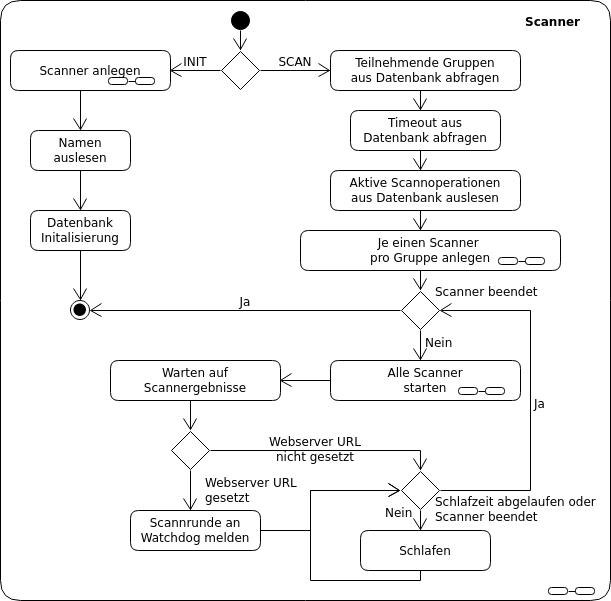
\includegraphics[width=\linewidth]{entwurf/scanner/state_scanner}
	\captionof{figure}{Ansicht des Scanners (Zustandsdiagramm)}
	\label{fig:scanner-state}
\end{center}

Bei Starten des Scanners wird die zu bearbeitende Aufgabe spezifiziert.

Bekommt der Scanner die Aufgabe \textquote{INIT}, soll dieser die Datenbank Service mit den implementierten Scan-Operationen füllen, sodass Administrierende diese an- oder ausschalten können. Um die Datenbank Service zu füllen, wird zunächst ein Dummy der Klasse Scanner angelegt. Aus diesem Objekt werden von allen Scan-Operationen der Anzeigename und der interne Name ausgelesen. Nach dem Auslesen alle Operationen werden die erhaltenen Daten gebündelt in die Datenbank geschrieben. Danach beendet der Scanner die Verbindung zur Datenbank und endet erfolgreich mit dem Statuscode 0.

Falls die Aufgabe des Scanners \textquote{SCAN} ist, wird der Scan der GameClients gestartet. Hierzu werden die teilnehmenden Gruppen und das Intervall der Scandurchgänge aus der Datenbank ausgelesen. Neben diesem werden die aktiven Scanner aus der Datenbank abgefragt. Sind alle Informationen vorhanden, wird für jede Gruppe ein Objekt der Klasse Scanner erstellt. Bei der Erstellung werden die aktiven Scan-Operationen sowie die zu überwachende Gruppe übergeben. Das Objekt legt dann für die benötigten Scan-Operationen die jeweiligen Objekte an.

\begin{center}
	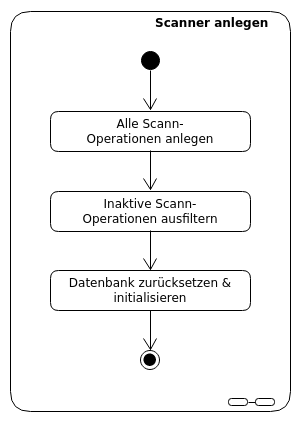
\includegraphics{entwurf/scanner/state_scanner_create}
	\captionof{figure}{Erstellung eines Scanners (Zustandsdiagramm)}
	\label{fig:scanner-create-state}
\end{center}

Nach dem Anlegen aller Scanner wird die Methode \textit{start()} parallel gestartet. Im Anschluss wird auf das Beenden der gestarteten Methoden gewartet. Sollten alle abgeschlossen sein, wird geprüft, ob das Durchführen einer Scan-Runde an den Webserver gemeldet werden soll. Ist dies der Fall, wird der Server darüber in Kenntnis gesetzt, dass neue Daten in der Datenbank vorhanden sind. Danach schläft der Scanner bis zum nächsten Durchlauf.

\begin{minipage}{\textwidth}
	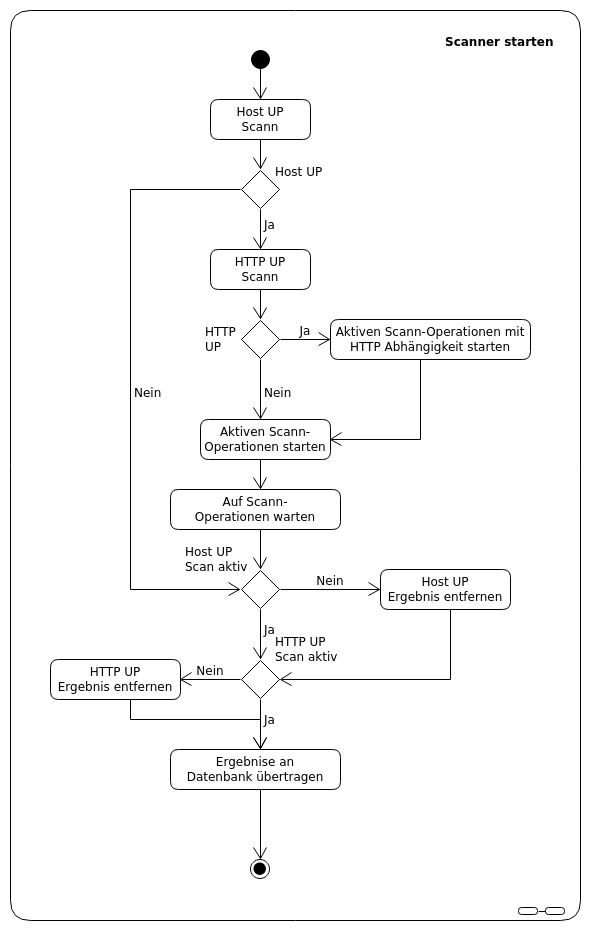
\includegraphics[height=\textheight]{entwurf/scanner/state_scanner_start}
	\captionof{figure}{Starten eines Scanners (Zustandsdiagramm)}
\end{minipage}

Beim Ausführen der Methode \textit{start()} des Scanners wird zunächst geprüft, ob das entfernte System erreichbar ist. Sollte dies nicht der Fall sein, werden alle nachfolgenden Scan-Operationen nicht durchgeführt, da diese fehlschlagen würden. Im Anschluss wird getestet, ob der HTTP-Dienst des entfernten Systems erreichbar ist, da dieser für einige weitere Tests benötigt wird. Ist der HTTP-Dienst erreichbar, werden die Scan-Operationen, welche auf dem HTTP-Dienst basieren, mit in die Liste der abzuarbeitenden Scan-Operationen aufgenommen. Danach werden alle verbleibenden Scan-Operationen parallel gestartet. Nachdem die Scan-Operationen ihre Aufgabe abgeschlossen haben, sammelt der Scanner alle Ergebnisse ein. Falls die \textit{Host UP Scan-Operation} oder die \textit{HTTP UP Scan-Operation} deaktiviert sind, werden diese aus dem Ergebnis entfernt. Danach übermittelt der Scanner die gesammelten Ergebnisse an die Datenbank und beendet seine Scan-Runde.

\subsection{Scan-Operationen}

Die Scan-Operationen werden parallel abgearbeitet, um so die Dauer eines kompletten Scans zu minimieren. Eine Scan-Operation prüft genau einen Dienst beziehungsweise eine Schwachstelle auf dem entfernten Rechner. Die im alten System implementieren Scans werden in die Scan-Operationen überführt. Deshalb sollen die folgenden Scan-Operationen implementiert werden.

\begin{itemize}
	\item Host-Up \\
	prüft, ob der entfernte Rechner mithilfe von ICMP Paketen erreichbar ist
	\item Bubble-Up \\
	prüft, ob der Bubble-Server erreichbar ist und ob die Telnet Steuerung funktioniert
	\item BubbleNg-Up\\
	prüft, ob der Bubble-NG-Server erreichbar ist und ob die Telnet Steuerung funktioniert
	\item FTP-Save\\
	prüft, ob der FTP-Server erreichbar und ob die Nutzung des anonymen Logins unterbunden worden ist
	\item Htaccess-Save\\
	prüft, ob die Kombination aus Nutzername und Passwort des Htaccess-Schutzes geändert wurde
	\item SQL-Injection-Save\\
	prüft, ob die SQL-Injection im Login zum Membersbereich verhindert wurde
	\item SQL-Password-Save\\
	prüft, ob das lokale Passwort des SQL-Nutzers root geändert wurde
	\item Telnet-Save\\
	prüft, ob der Telnet Server deaktiviert bzw. deinstalliert wurde
	\item HTTP-UP\\
	prüft, ob der HTTP Dienst des entfernten Rechners nutzbar ist
	\item HTTPS-UP\\
	prüft, ob der HTTPS Dienst des entfernten Rechners nutzbar ist
	\item XSS-Save\\
	prüft, ob der Cross-Site-Scripting Angriff im Bewertungsformular behoben wurde.
\end{itemize}

\begin{center}
	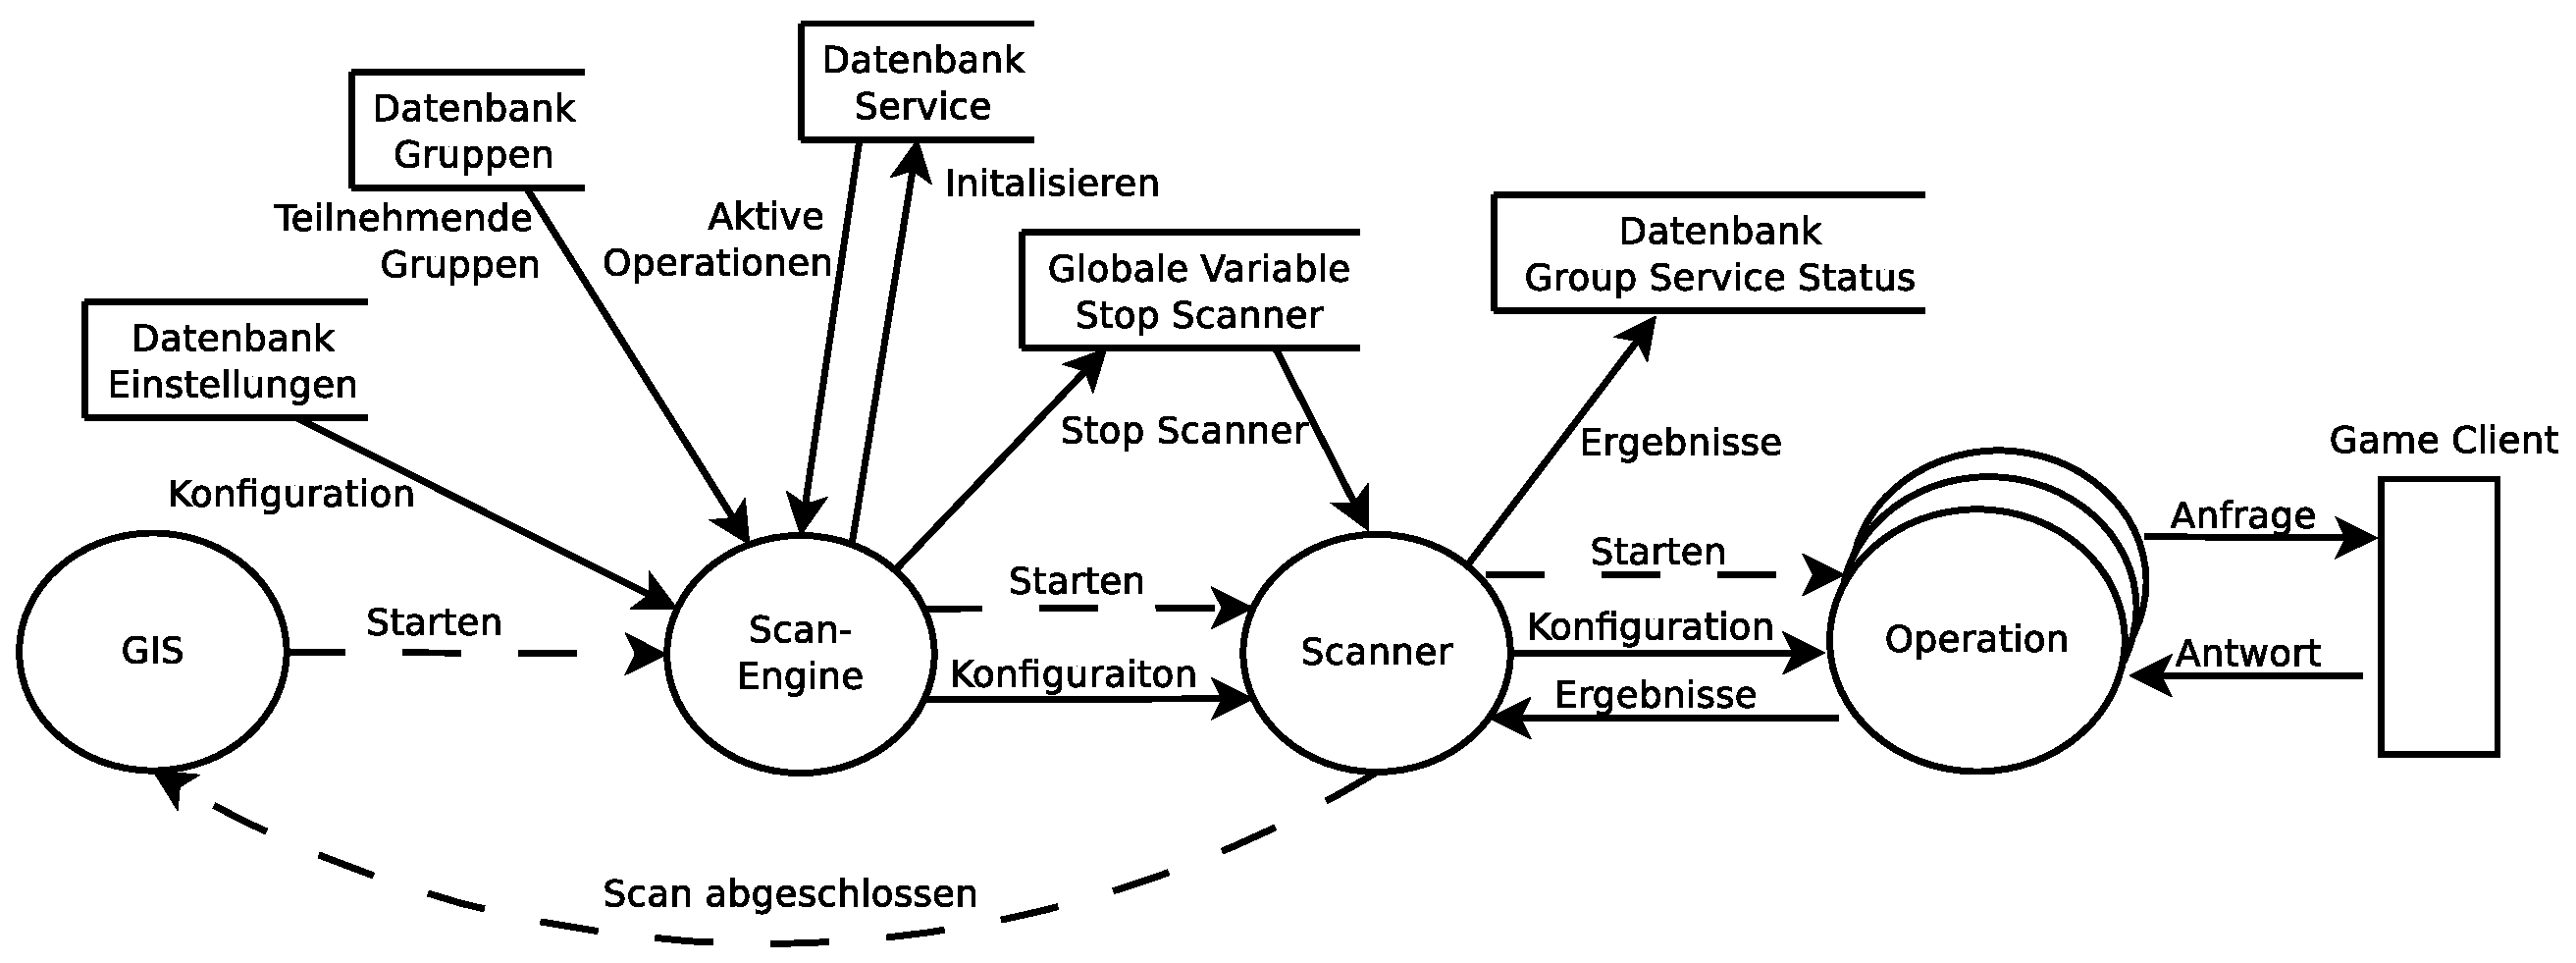
\includegraphics[width=\linewidth]{entwurf/scanner/dfd-scanner}
	\captionof{figure}{Datenfluss in der Scanner Komponente (Datenflussdiagramm)}
	\label{fig:dfd-scanner}
\end{center}

Die im Datenflussdiagramm (\autoref{fig:dfd-scanner}) sichtbaren, aber bisher nicht beschriebenen Datenflüsse finden zwischen dem Webserver und dem Scanner oder einer Scan-Operation und dem GameClient statt. Administrierende und betreuende Personen können über den Webserver den Scanner an- und abschalten. Die Scan-Operationen fragen bei dem GameClient ihren überwachten Dienst beziehungsweise ihre überwachte Schwachstelle an und erhalten eine Antwort zurück. Anhand dieser wird das Ergebnis der Scan-Operationen bestimmt.